\chapter{Avaliação}

Neste capítulo, será mostrado os resultados da aplicação do software em um contexto real, ou seja, o software foi
utilizado na disciplina de Teste de Software do curso de engenharia de software na universidade de brasília campus
de engenharias gama. O capítulo está dividido em seções que estão disposta da seguinte maneira: na seção 5.1 será mostrado
uma pequena introdução sobre os questionários de avaliação, na seção 5.2 será listado os cenários de avaliação, na
seção 5.3 será mostrado o questionário de avaliação e na seção 5.4 o resultado da avaliação.

\section{Questionários de Usabilidade}

Uma parte importante da engenharia de produtos é a medida de usabilidade. Os métodos de medição para avaliar a
usabilidade não são óbvios e são um preocupação permanente dos engenheiros. A maioria das avaliações de usabilidade
reúne dados quantitativos subjetivos e objetos no contexto de cenários realistas de uso. Os dados subjetivos são medidas
das opiniões ou atitudes dos participantes em relação a sua percepção de usabilidade, já os objetivos são medidas do
desempenho dos participantes como tempo de conclusão, taxa de sucesso e etc \cite{questionario}.

Como o objetivo do software é automatizar e aumentar a satisfação do uso de metodologias ativas de aprendizado, as
medidas subjetivas terão maior consideração na avaliação do mesmo. As medidas subjetivas são geralmente respostas a
itens do questionário do tipo "\textit{like}" que avaliam atitudes do usuário em relação a atributos como facilidade de uso do
sistema e a similaridade de interfaces em determinados cenários. A maioria dos cenários de avaliação de usabilidade são
conjuntos de tarefas nas quais os usuários resolvem problemas, por exemplo, como resolver a lista de exercício, se
preparando para as avaliações, automatizar o cálculo das notas entre outras em relação aos requisitos não funcionais \cite{questionario}.

Para adquirir essas métricas será utilizado um questionário da IBM especificamente para uso no contexto de testes de
usabilidade baseados em cenários e medidas subjetivas. Foi analisado alguns tipos de questionários como o
\textit{After-Scenario Questionnaire} (ASQ), \textit{Printer Scenario Questionnaire} (PSQ), \textit{Post-Study System
Usability Questionnaire} (PSSUQ) e \textit{Computer System Usability Questionnaire} (CSUQ). Como as metodologias ativas
de aprendizado tem alguns cenários que precisam ser avaliados separadamente, foi definido para a avaliação de satisfação
dos usuários o questionário ASQ, pois ele é um questionário curto e consegue adquirir métricas para cada cenário do
software. Apesar de o ASQ e o PSQ terem os mesmo itens mudando apenas a escala de avaliação, o ASQ tem uma
confiabilidade melhor de acordo com \cite{questionario}. Já o PSSUQ e o CSUQ são ambos questionários gerais de
satisfação, ou seja, são questionários mais extensos que englobam todo o sistema, que não é o ideal para a avaliação, já
que não conseguiria coletar feedbacks de cada cenário para possíveis melhorias.

\section{Cenários de avaliação}

Abaixo será listado os cenários de avaliação na qual será aplicado o questionário ASQ em comparação ao mesmo cenário sem
utilizar o softwate PGTBL.

\begin{itemize}
  \item avaliação iRAT
  \item avaliação gRAT
\end{itemize}

Os 2 itens são questionários para o estudante responder depois de cada cenário.

\section{Questionário ASQ}

O questionário Pós-cenário (ASQ) é um questionário de três ou mais itens que os avaliadores de usabilidade da IBM utilizam para
avaliar a satisfação do participante após a conclusão de cada cenário proposto \cite{questionario}. Os itens do
questionário abordam afirmações relacionadas a 4 dos 5 requisitos não funcionais aplicados a ferramenta para avaliar se
os requisitos foram satisfeitos. Os requisitos são: suportabilidade, desempenho, usabilidade e segurança ou
confiabilidade. O quinto requisito não funcional, o requisito de qualidade, é respondido pelas métricas
coletadas na ferramenta codacy.

O questionário será constituido de itens com escalas gráficas de 7 pontos, na qual temos 7 para o caso do usuário concordar
totalmente e 1 caso discordar totalmente e um ponto não aplicavel (N/A) fora da escala para o caso de o usuário não
querer responder. O resultado será a média aritmética dos escores dos quatro itens para obter a pontuação do ASQ para a
satisfação de um participante com o sistema para um determinado cenário. Quanto mais alto o resultado melhor. Se um
participante não responder a um item ou marcar N/A, o cálculo da média será a média dos itens respondidos.

$$P_{i} = \frac{x_{1} + x_{2} + x_{3} + x_{4}}{4}$$

$$R_{req} = \sum_{i=1}^{n} \frac{y_{i}}{n}$$

$$R_{final} = \sum_{i=1}^{n} \frac{P_{i}}{n}$$

$P_i$ é a pontuação final de cada aluno no questionário, $x$ é a pontuação de cada item do questionário, $y$ é a nota do
aluno relacionada ao requisito não funcional especificado, $R_{req}$ é a média dos pontos para um determinado requisito
não funcional, $R_{final}$ é o resultado final da avaliação de usabilidade, $i$ é o indice de cada aluno e $n$ é a
quantidade total de alunos. A média padrão do questionário é 4.0, se o resultado da média relacionada ao requisito não
funcional tiver abaixo dessa média padrão, o requisito não foi satisfeito, e se o resultado final de um determinado cenário
tiver abaixo da média padrão, quer dizer que o cénario não foi bem aceito.

Questionário para cada cenário:

Em relação ao software PGTBL para cada uma das afirmações abaixo, preencha a classificação de sua escolha.

\begin{figure}[h!]
  \centering
  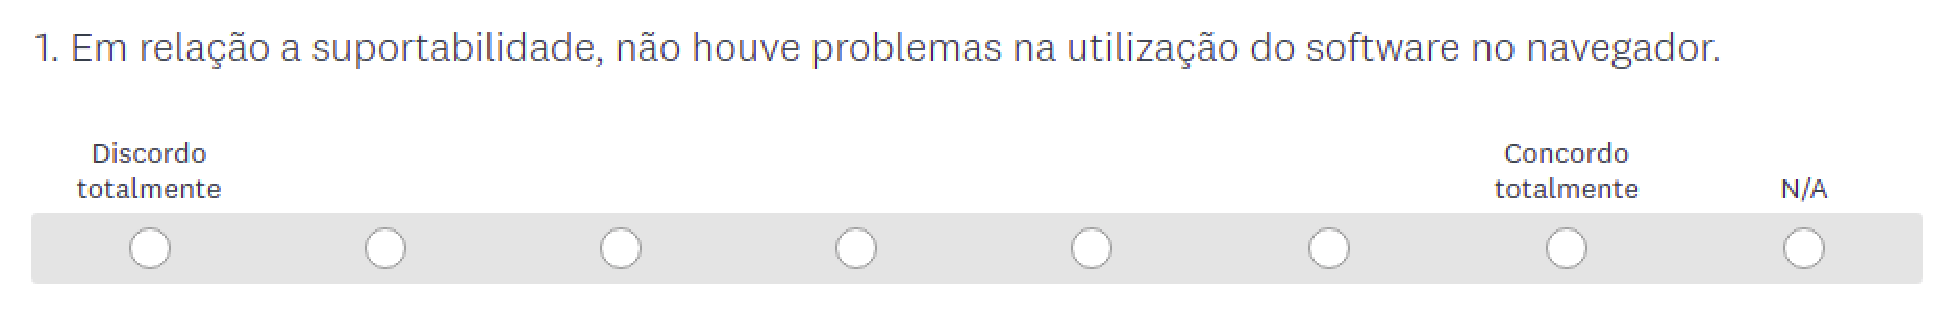
\includegraphics[keepaspectratio=true,scale=0.5]{figuras/p1.eps}
\end{figure}

\begin{figure}[h!]
  \centering
  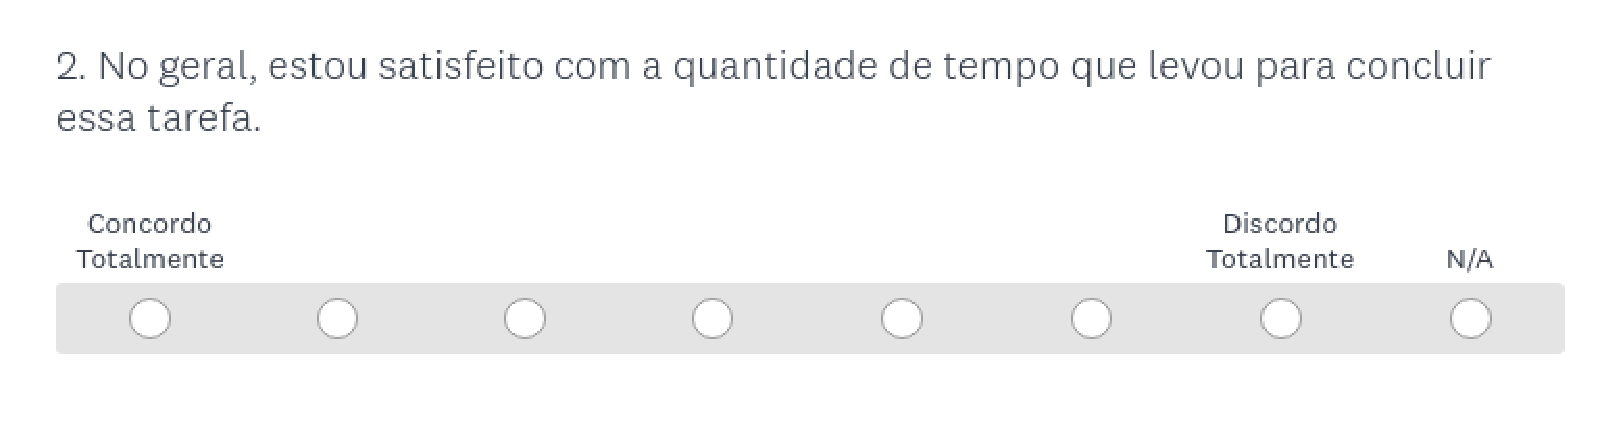
\includegraphics[keepaspectratio=true,scale=0.5]{figuras/p2.eps}
\end{figure}

\begin{figure}[h!]
  \centering
  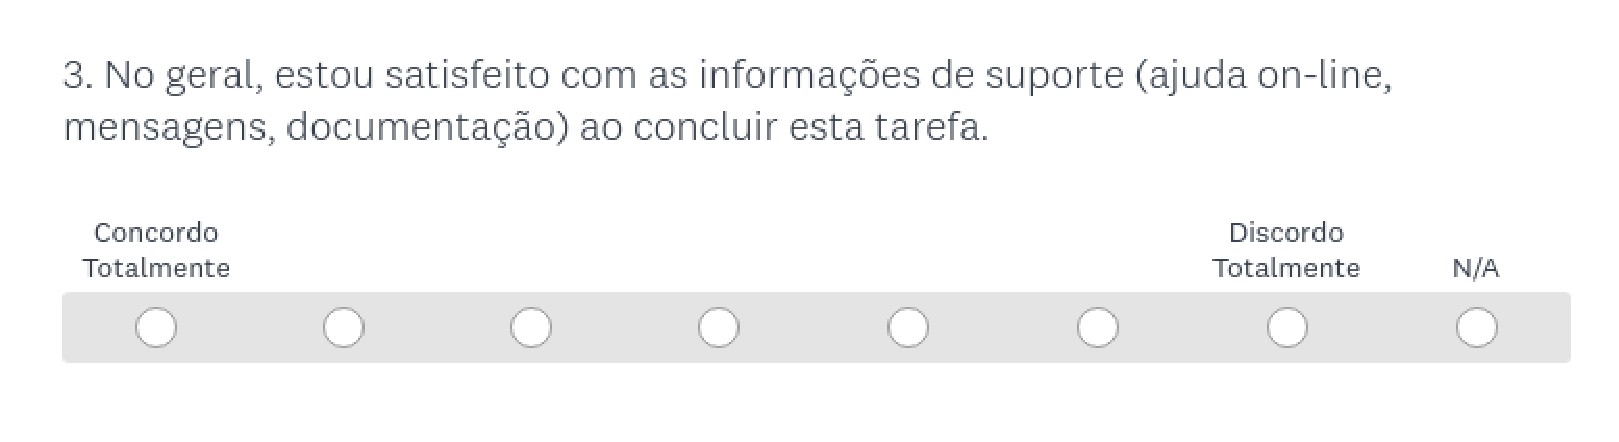
\includegraphics[keepaspectratio=true,scale=0.5]{figuras/p3.eps}
\end{figure}

\begin{figure}[h!]
  \centering
  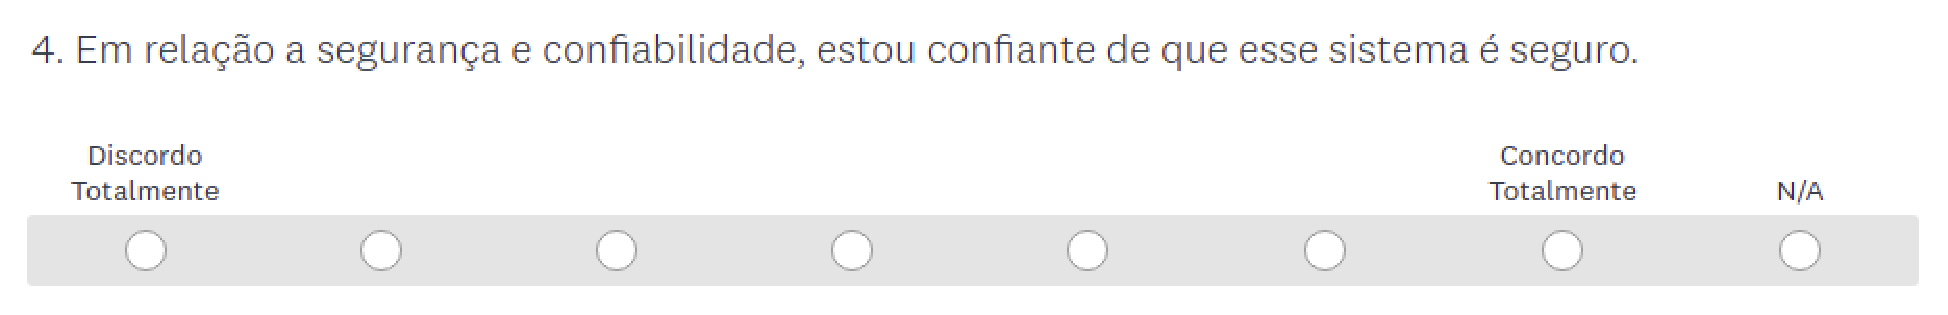
\includegraphics[keepaspectratio=true,scale=0.5]{figuras/p4.eps}
\end{figure}

\section{Resultado}

Nesta seção será apresentado os resultados do estudo de cado para os dois cenários especificados: iRAT e gRAT. Os outros
cenários como Avalição prática e avaliação em pares não foi possível de ser feito por limitações no servidor de
produção.

\subsection{Objetivo}

Normalmente os alunos tem um pouco de dificuldade em aceitar o novo e sair do comodismo, que são as avaliações no papel, como foi explicado no referência
teórico do trabalho, isso pode dificultar um pouco a aceitação da ferramenta, já que, por ser algo
novo e está sendo aplicado a uma disciplina em que a menção é importante para a continuação do curso por parte do aluno.
A ferramenta pode trazer um pouco de desconforto

O objetivo dessa avaliação é verificar o indice de usabilidade para cada um dos requisitos não funcionais dentro do
contexto dos cenários propostos.

\subsection{Roteiro}

No dia 03/06/2019 será realizado a avaliação iRAT e gRAT do TBL2 da disciplina de teste de software na universidade de brasília utilizando a ferramenta.

O questionários será realizado da seguinte maneira:

\begin{enumerate}
  \item Antes da avaliação os alunos serão cadastrados na ferramenta e inseridos na disciplina.
  \item Com os alunos cadastrados, o professor irá montar os grupos na ferramenta e disponibiliza-los para os alunos.
  \item No dia 03/06/2019 às 14:30 a avaliação iRAT será disponibilizada e terá duração de 30 minutos.
  \item No mesmo dia de 15:00 às 15:10 será o tempo para os alunos responderem o questionário voltado ao iRAT
  \item No mesmo dia de 15:20 às 15:40 será liberado a avaliação gRAT em que apenas um aluno junto com seu grupo irá submeter.
  \item No mesmo dia de 15:40 às 16:00 será o tempo para os alunos responderem o questionário voltado ao gRAT e visualizar sua nota na ferramenta.
  \item Às 16:00 se encerra a avaliação e é recolhido os questionários e gerado o relatório na ferramenta para o professor.
\end{enumerate}

\subsection{Resultados Esperados}

Na questão sobre portabilidade, pode-se esperar que o resultado seja positivo, entre 5 e 7, já que a ferramenta é voltada para o
navegado que é suportado em qualquer sistema operacional, em qualquer computador. Na segunda questão voltada ao
desempenho para a realização da tarefa, aqui terá convergencias e divergencias já que o maior foco da ferramenta no
quesito de agilidade é para o professor no cálculo das notas, e na economia de recursos.

Na terceira questão voltado a usabilidade da ferramente, espera-se um valor alto entre 5 e 7, já que a ferramenta foi
desenhada para ser fácil de usar, padronizado e com um design atraente. Na última questão voltado a segurança e
confiabilidade da ferramenta, não se espera um resultado muito posítivo já que os alunos normalmente tem um pouco de
dificuldade de aceitar o novo, principalmente quando se trata de avaliação.

\subsection{Resultados Obtidos iRAT}

\begin{figure}[H]
	\centering
  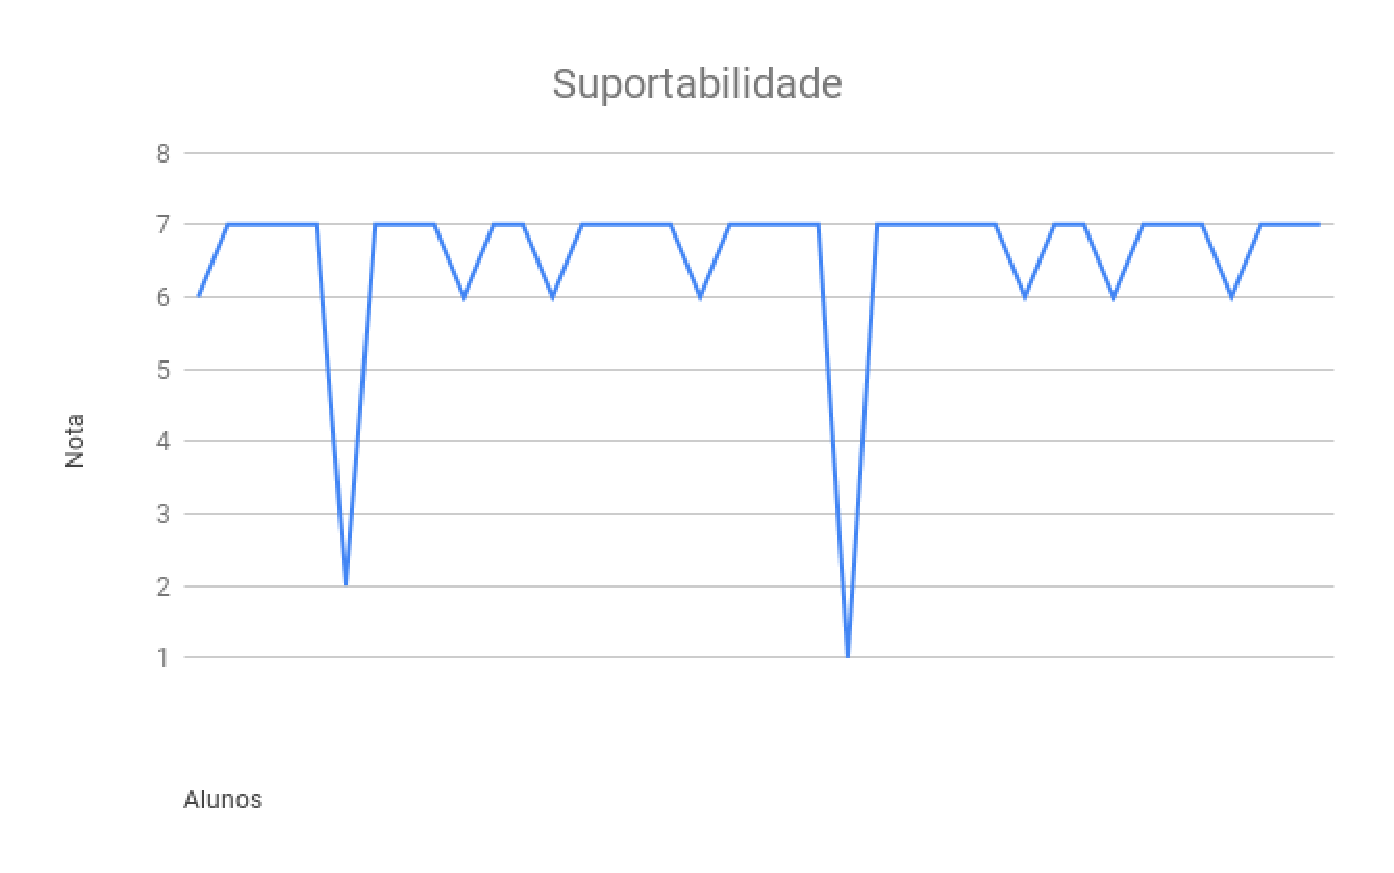
\includegraphics[keepaspectratio=true,scale=0.5]{figuras/iRAT_Suportabilidade.eps}
  \caption[iRAT Suportabilidade.]{iRAT Suportabilidade. Fonte: Autor}
\end{figure}

\textbf{Análise}: A média obtida desse requisito não funcional foi de 6.54, como citado anteriormente já era
esperado esse tipo de resultado.

\begin{figure}[H]
	\centering
  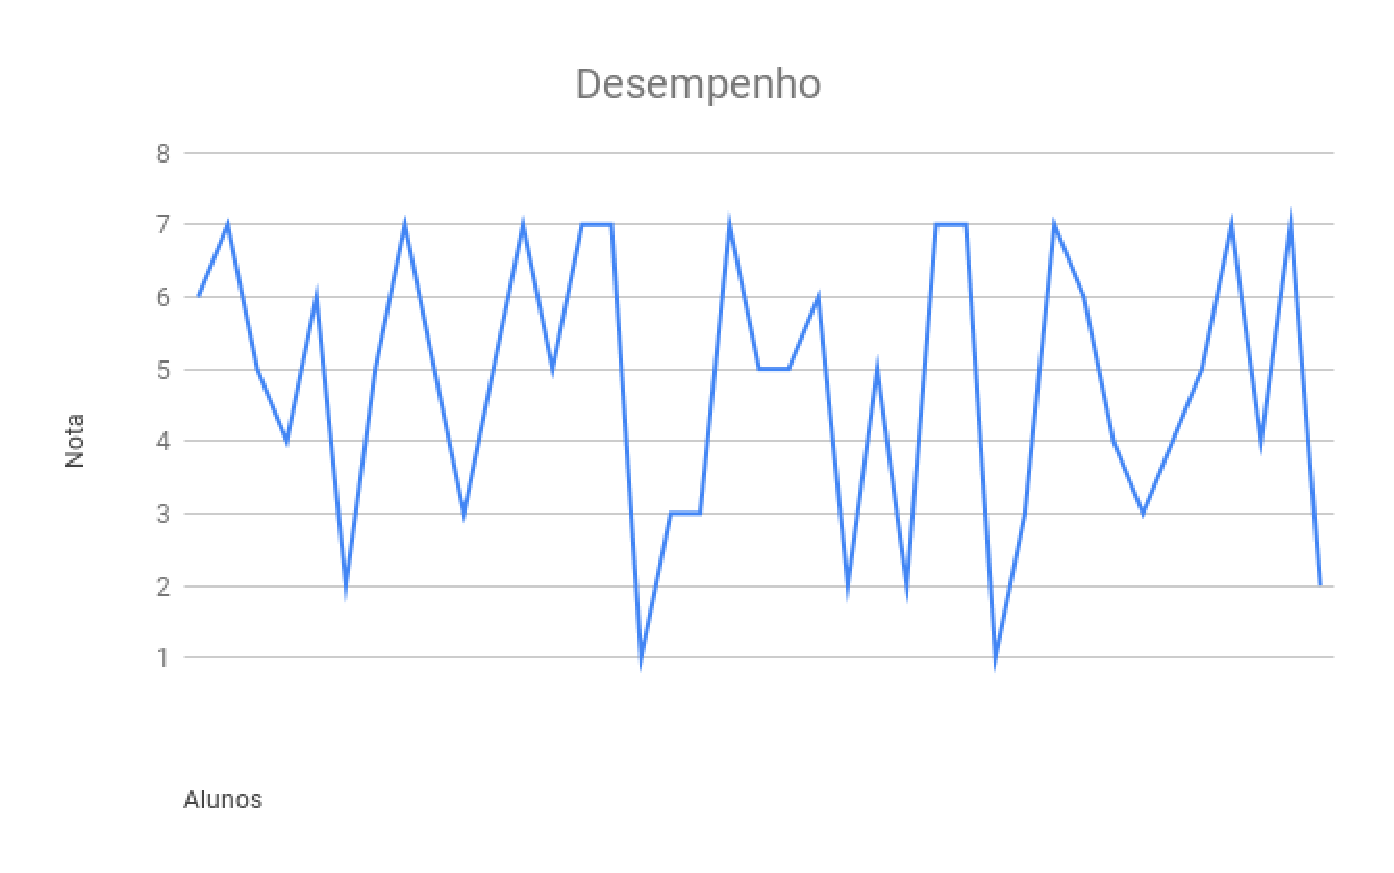
\includegraphics[keepaspectratio=true,scale=0.5]{figuras/iRAT_Desempenho.eps}
  \caption[iRAT Desempenho.]{iRAT Desempenho. Fonte: Autor}
\end{figure}

\textbf{Análise}: A média obtida desse requisito não funcional foi de 4.79, como citado anteriormente o
resultado do requisito de desempenho iria oscilar bastante no gráfico, e o resultado ficou um pouco acima da média
  padrão.

\begin{figure}[H]
	\centering
  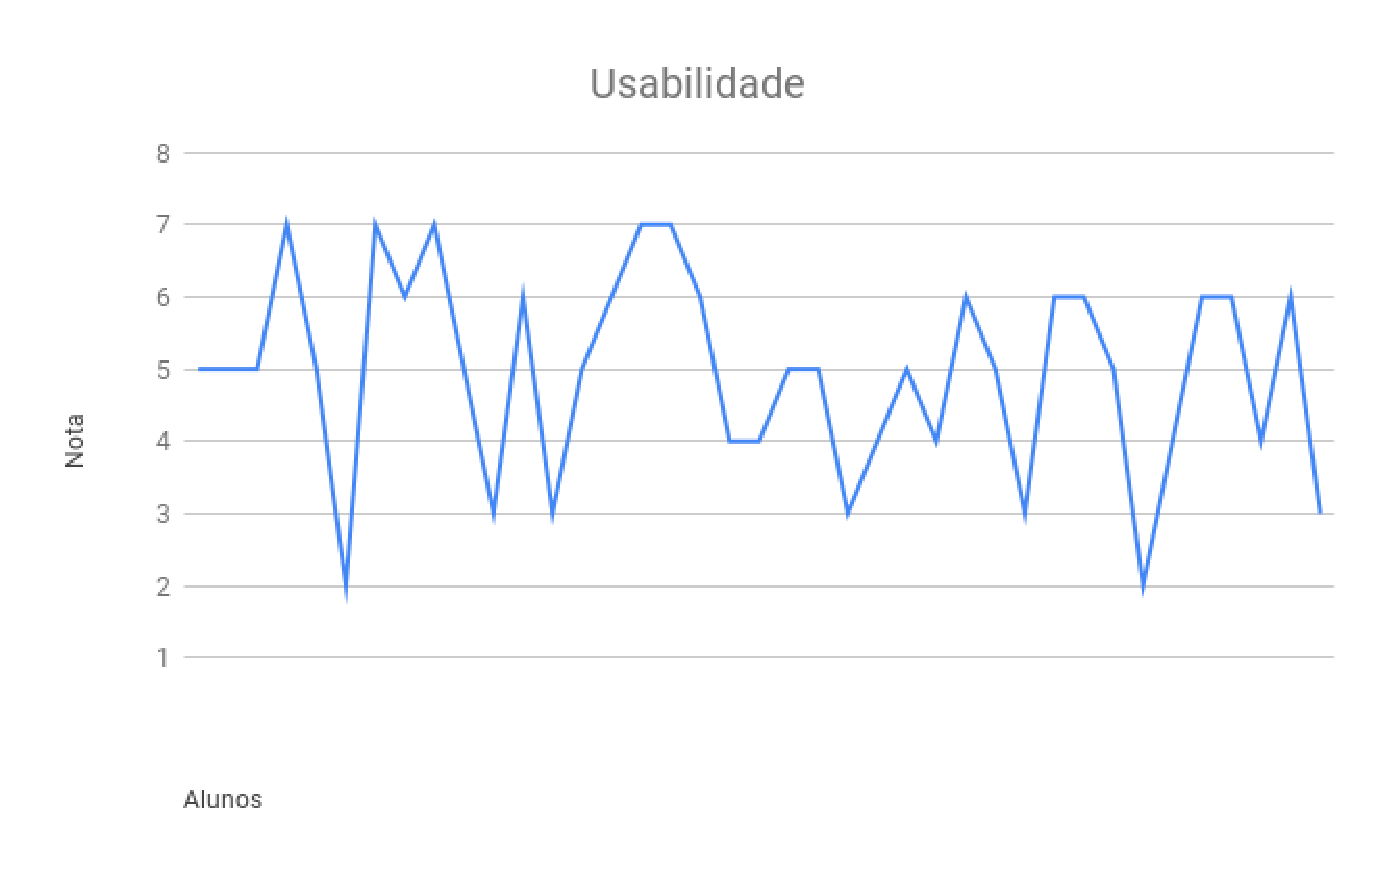
\includegraphics[keepaspectratio=true,scale=0.5]{figuras/iRAT_Usabilidade.eps}
  \caption[iRAT Usabilidade.]{iRAT Usabilidade. Fonte: Autor}
\end{figure}

\textbf{Análise}: A média obtida desse requisito não funcional foi de 4.95, erá esperado um resultado maior para
esse requisito não funcional, porém ainda está acima da média padrão.

\begin{figure}[H]
	\centering
  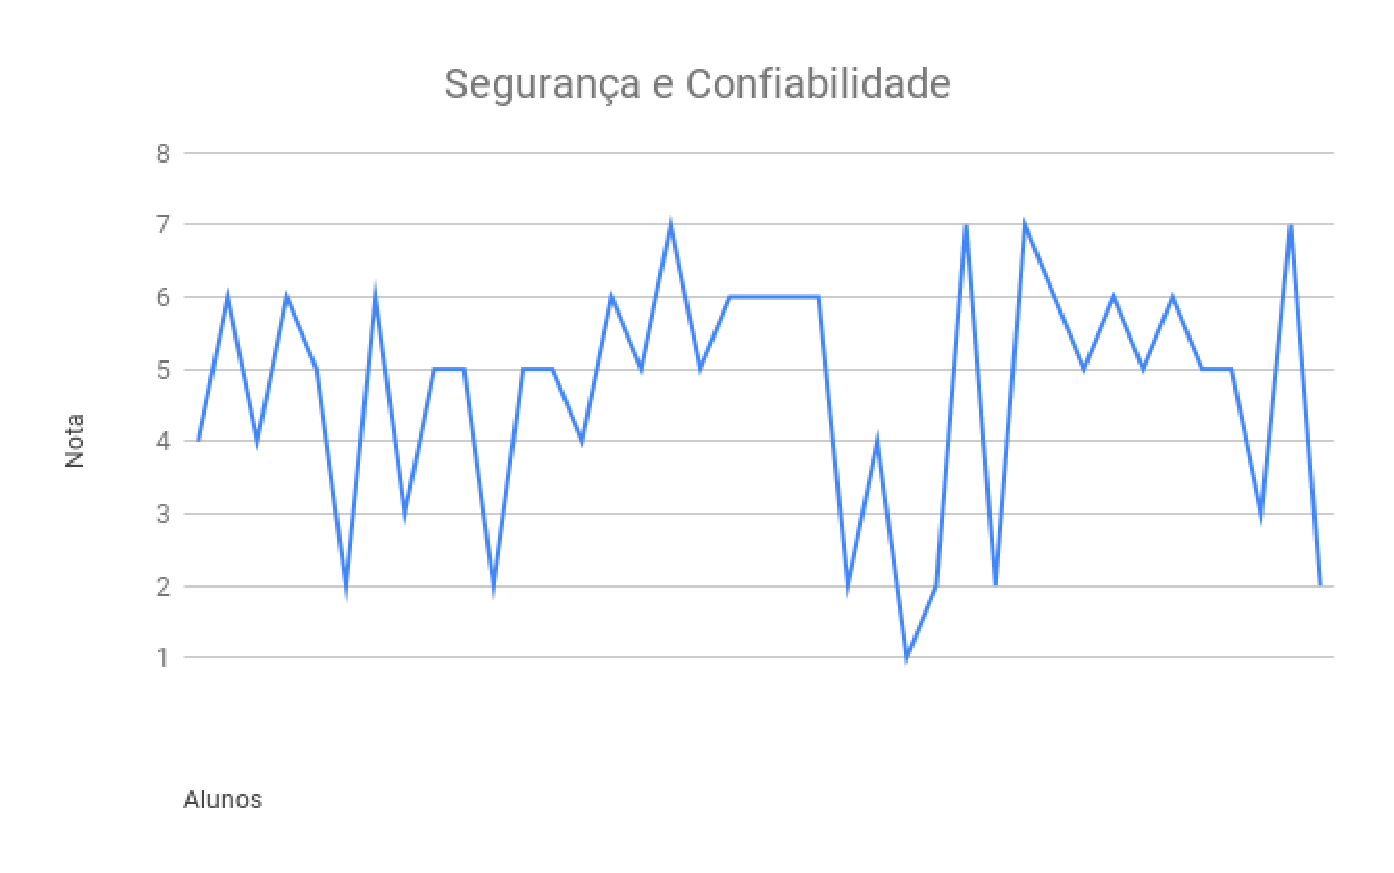
\includegraphics[keepaspectratio=true,scale=0.5]{figuras/iRAT_Seguranca_e_Confiabilidade.eps}
  \caption[iRAT Segurança e Confiabilidade.]{iRAT Segurança e Confiabilidade. Fonte: Autor}
\end{figure}

\textbf{Análise}: A média obtida desse requisito não funcional foi de 4.72, erá esperado um resultado menor, porém o
resultado foi acima de média padrão.

\begin{figure}[H]
	\centering
  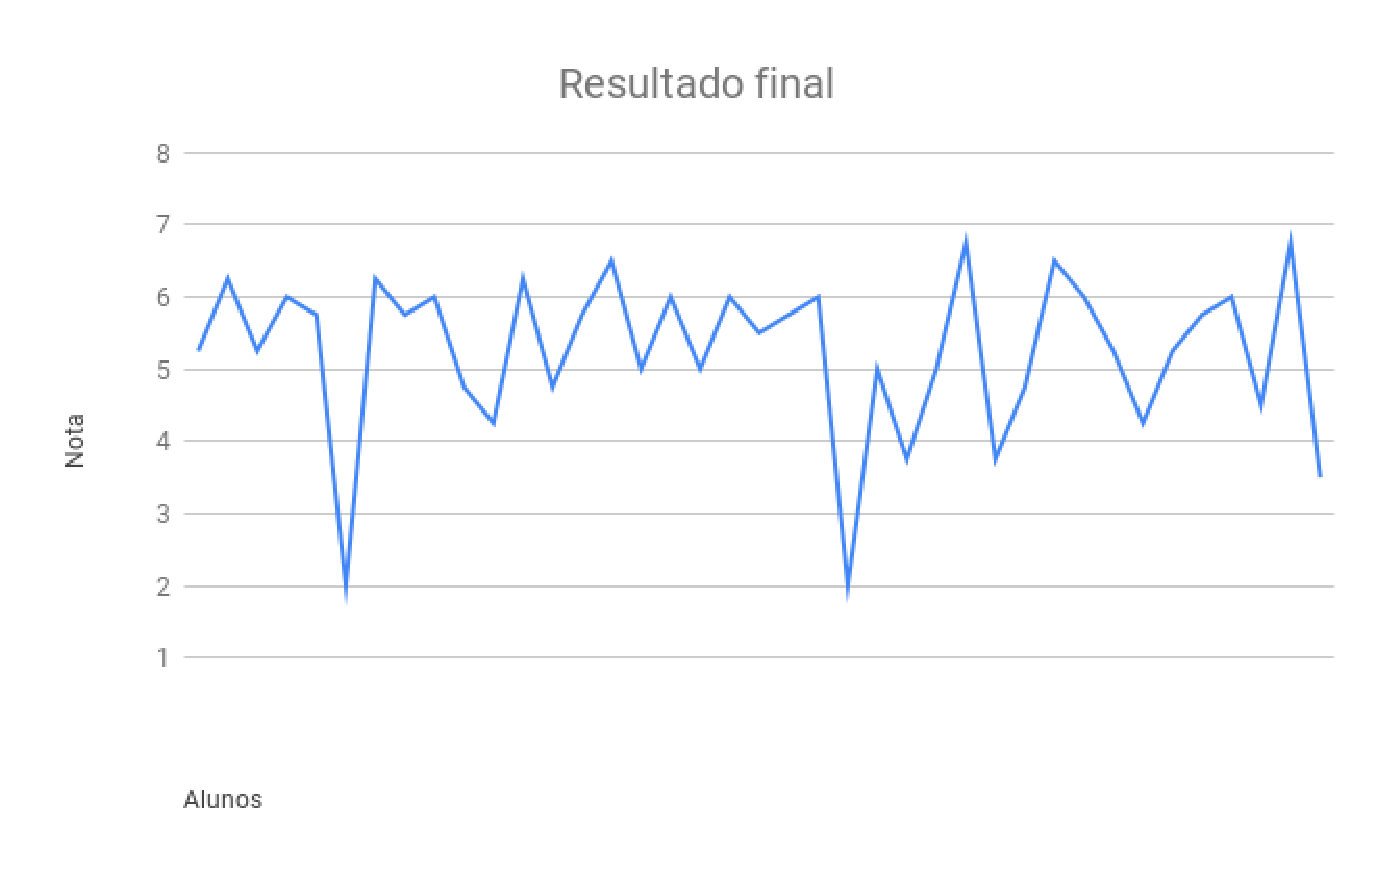
\includegraphics[keepaspectratio=true,scale=0.5]{figuras/iRAT_Resultado_Final.eps}
  \caption[iRAT Resultado Final.]{iRAT Resultado Final. Fonte: Autor}
\end{figure}

\textbf{Análise}: A média obtida desse requisito não funcional foi de 5.25, ou seja, o iRAT teve uma avaliação
positiva em relação os requisitos não funcionais especificados.

\subsection{Resultados Obtidos gRAT}

\begin{figure}[H]
	\centering
  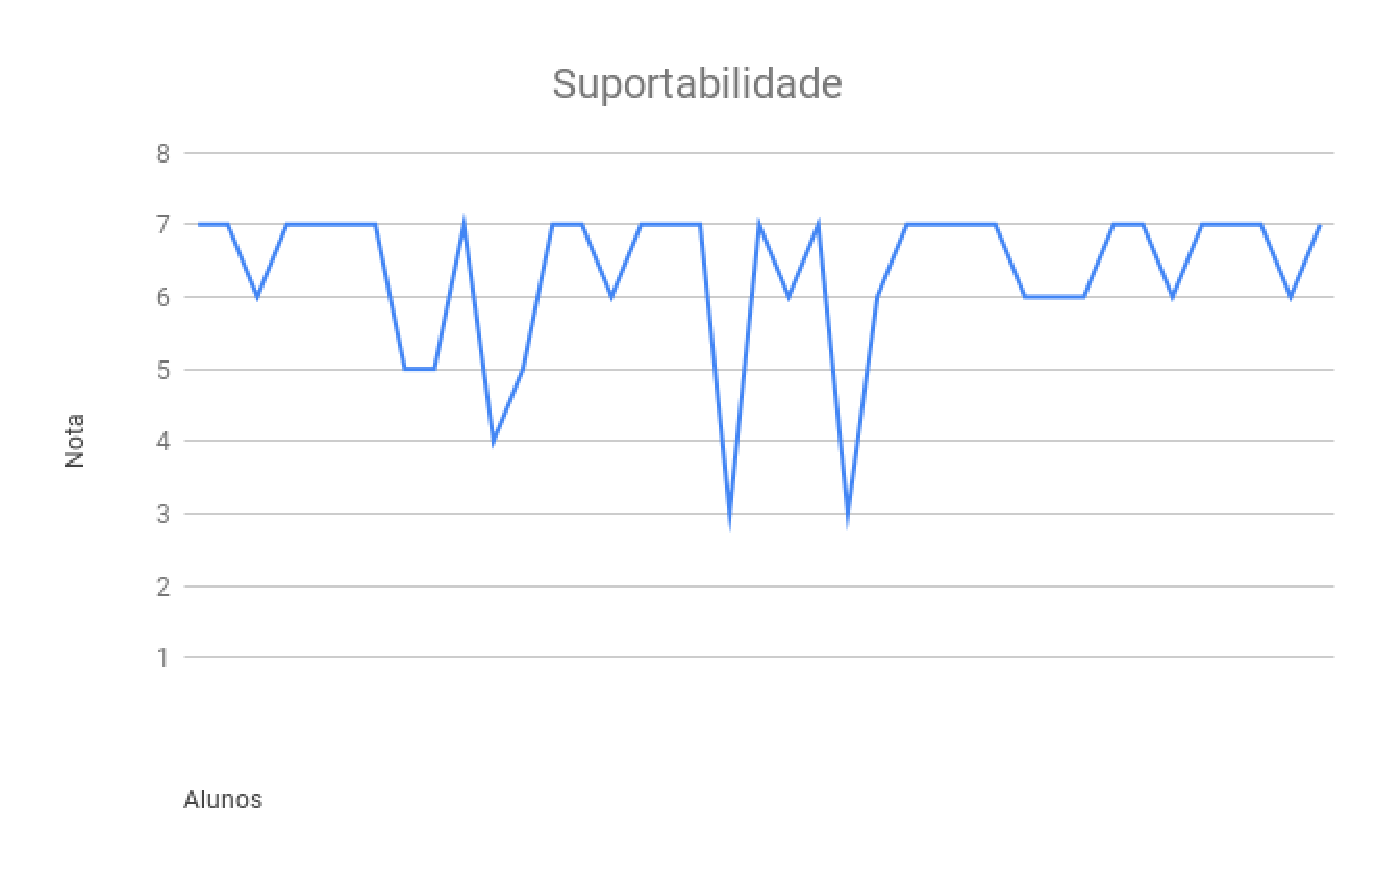
\includegraphics[keepaspectratio=true,scale=0.5]{figuras/gRAT_Suportabilidade.eps}
  \caption[gRAT Suportabilidade.]{gRAT Suportabilidade. Fonte: Autor}
\end{figure}

\textbf{Análise}: A média obtida desse requisito não funcional foi de 6.33, assim como o iRAT já era
esperado esse tipo de resultado.

\begin{figure}[H]
	\centering
  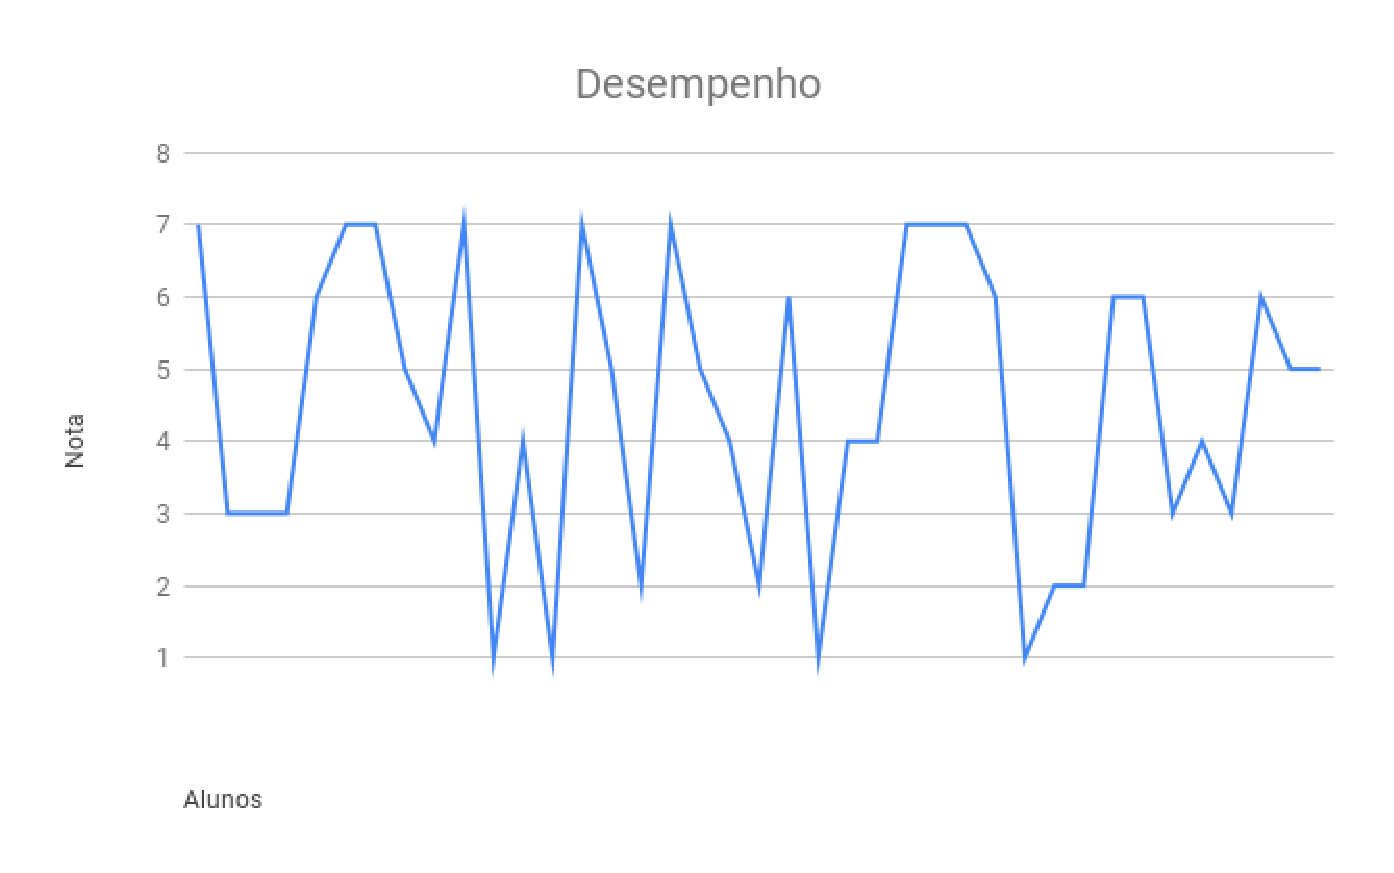
\includegraphics[keepaspectratio=true,scale=0.5]{figuras/gRAT_Desempenho.eps}
  \caption[gRAT Desempenho.]{gRAT Desempenho. Fonte: Autor}
\end{figure}

\textbf{Análise}: A média obtida desse requisito não funcional foi de 4.49, assim como o iRAT o
resultado do requisito de desempenho iria oscilar bastante no gráfico, e o resultado ficou um pouco acima da média
  padrão.

\begin{figure}[H]
	\centering
  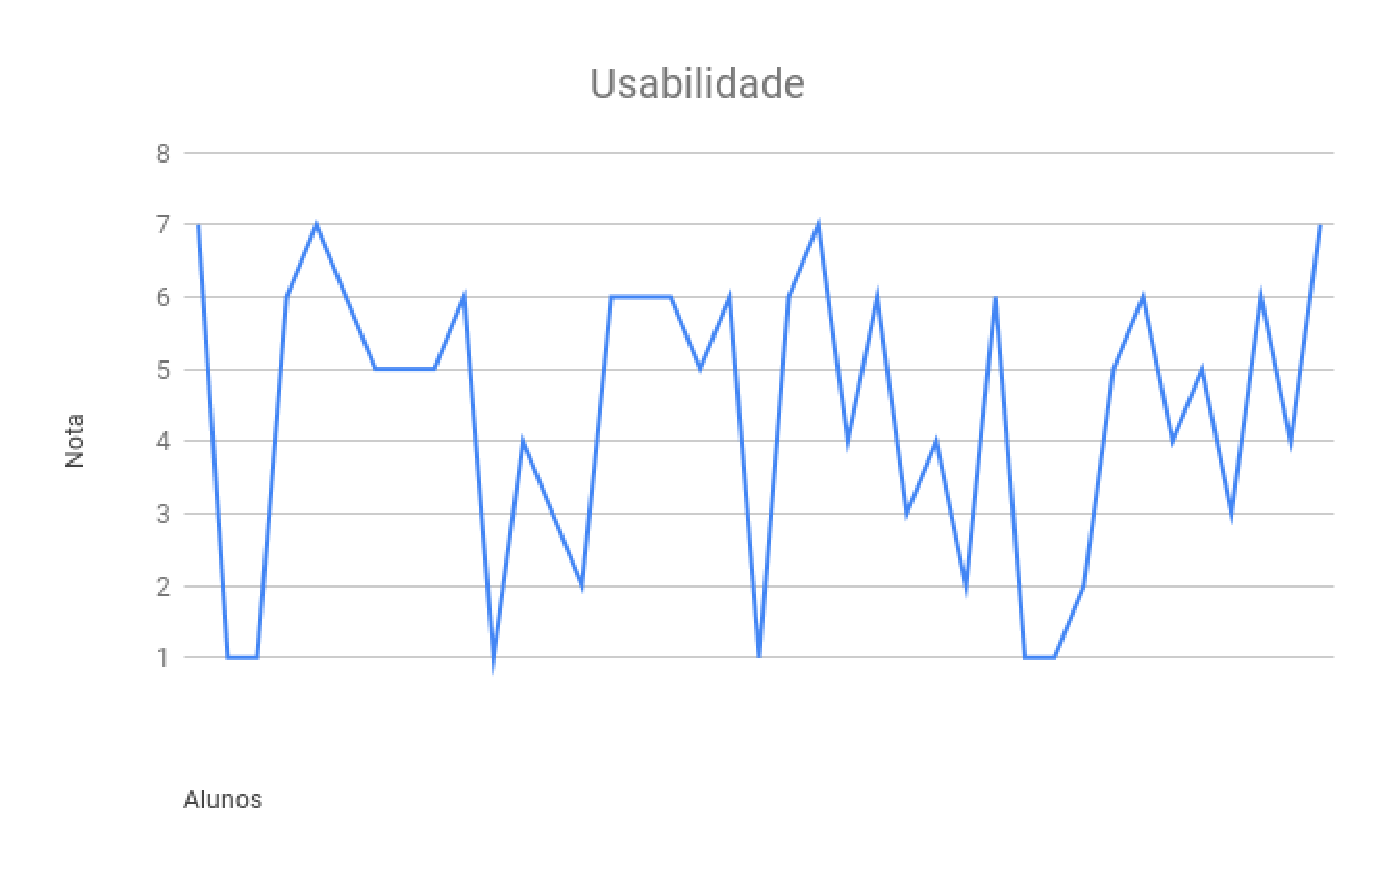
\includegraphics[keepaspectratio=true,scale=0.5]{figuras/gRAT_Usabilidade.eps}
  \caption[gRAT Usabilidade.]{gRAT Usabilidade. Fonte: Autor}
\end{figure}

\textbf{Análise}: A média obtida desse requisito não funcional foi de 4.38, assim como o iRAT também erá esperado um resultado maior para
esse requisito não funcional, porém ainda está acima da média padrão.

\begin{figure}[H]
	\centering
  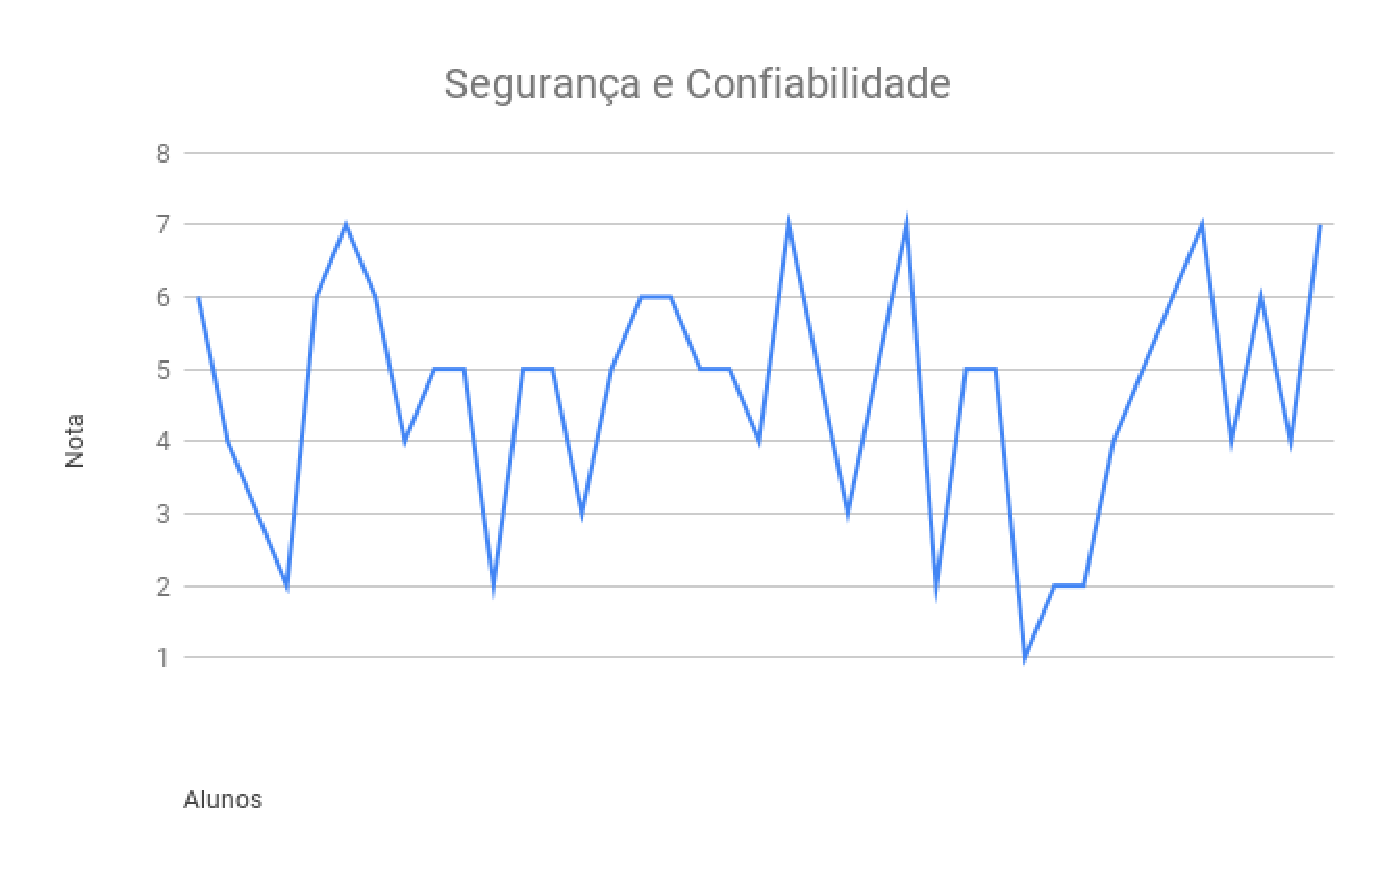
\includegraphics[keepaspectratio=true,scale=0.5]{figuras/gRAT_Seguranca_e_Confiabilidade.eps}
  \caption[gRAT Segurança e Confiabilidade.]{gRAT Segurança e Confiabilidade. Fonte: Autor}
\end{figure}

\textbf{Análise}: A média obtida desse requisito não funcional foi de 4.64, assim como no iRAT erá esperado um resultado menor, porém o
resultado foi acima da média padrão.

\begin{figure}[H]
	\centering
  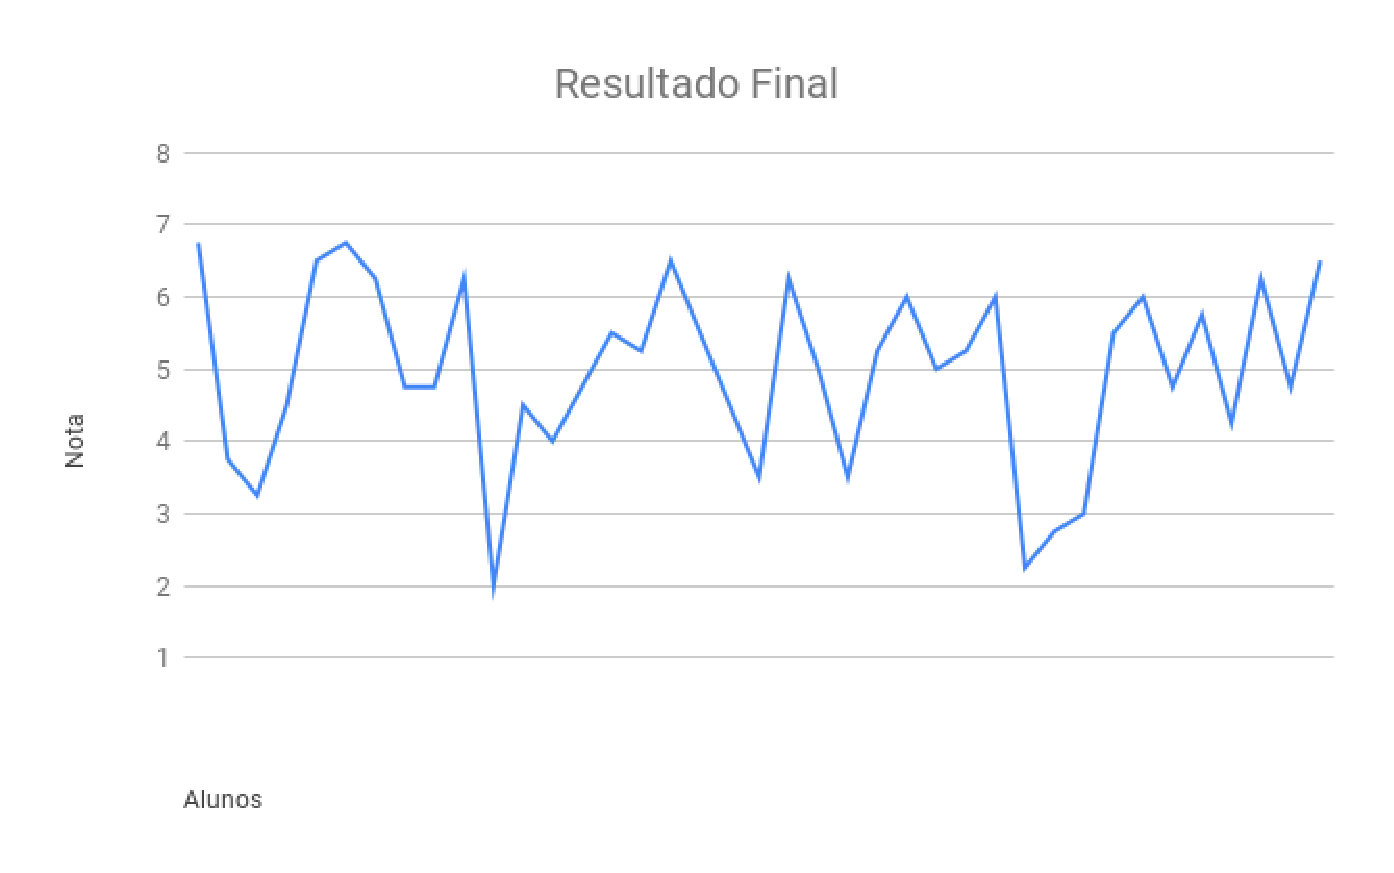
\includegraphics[keepaspectratio=true,scale=0.5]{figuras/gRAT_Resultado_Final.eps}
  \caption[gRAT Resultado Final.]{gRAT Resultado Final. Fonte: Autor}
\end{figure}

\textbf{Análise}: A média obtida desse requisito não funcional foi de 4.96, ou seja, o gRAT teve uma avaliação
positiva em relação os requisitos não funcionais especificados, porém um pouco menor do que a iRAT.

\subsection{Ponto de vista dos usuários}

O professor Ricardo Ajax, que utilizou a ferramenta em sua disciplina de teste de software, citou algumas
considerações sobre a experiência que ele teve usando a ferramenta:

\begin{quoting}[rightmargin=0cm, leftmargin=4cm]
  \noindent
  Esta é uma parte finalzinha, após o relato de termos usado o PGTBL em sala de aula para executar o TBL 2. Vamos a
  ele.

  \noindent
  O sistema foi usado para administrar toda uma seção completa de TBL e os resultado obtidos serviram como validação
  do uso do sistema junto aos seus usuários, além de coletar oportunidades de melhoria.

  \noindent
  Inicialmente foi feita uma seção onde todos os estudantes da turma se cadastraram no sistema. Para isso já tinha me
  cadastrado previamente, assim como criado a disciplina e a sessão de TBL a ser
  usada nos testes de validação do sistema. Os alunos foram acompanhados pelo desenvolvedor durante os seus
  cadastramentos, a fim de sanar alguma dúvida que ocorresse no cadastramento dos alunos, ou mesmo algum erro de
  sistema. Esta atividade ocupou certa de 30 a 40 minutos de uma das aulas da disciplina, cujo total de tempo é de 100
  minutos. Ou seja, foram ocupados cerca de 30 a 40\% de uma das aulas da disciplina, considerado um tempo bastante
  adequado para uma turma de 50 alunos. Posteriormente agrupamos os estudantes, preparando
  o PGTBL para ser usado na sessão onde o questionário é respondido em grupo.

  \noindent
  Dando continuidade aos testes de validação do sistema, inseri as questões da sessão de TBL a ser
  executado em sala de aula. Na inserção das questões, é necessário informar qual a alternativa correta de cada uma para
  que o sistema proceda com as devidas correções e atribuições de notas das várias fases do TBL. Esta atividade ocorreu
  sem maiores problemas. Algumas dúvidas pontuais sobre o uso das funcionalidades do sistema envolvidas com essa tarefa
  foram tiradas prontamente pelo desenvolvedor.  Com as questões prontas o tempo necessário para o cadastro delas no
  PGTBL foi considerado adequado (cerca de 1,5 a 2 minutos para cada questão) e não exitiram intercorrências na
  atividade . Ate esse momento todas as informações necessárias foram cadastradas no PGTBL, deixando-o pronto para a
  realização do TBL junto aos alunos.

  \noindent
  A sessão de TBL é realizada conforme cronograma de aulas da disciplina. Os estudantes devem estar em sala de aula com
  antecedência mínima de 15 minutos para que todas as máquinas sejam ligadas, o SISTEMA carregado e cada estudante
  esteja com o seu logon efetuado. Nos testes de validação esse tempo foi usado e a sessão de TBL só teve início quando
  todos os estudantes assinalaram estar logados ao sistema. Neste momento foi iniciado a sessão onde os alunos
  responderão individualmente o questionário (iRAT). A sessão tem tempo marcado que, após transcorrido o sistema encerra
  automaticamente a fase de respostas individuais.

  \noindent
  Após a sessão individual inicia-se a sessão onde os alunos respondem em grupo o questionário (gRAT).  A mesma
  dinâmica  de início e prazos marcados é usada, mas os alunos podem se dispor fisicamente conforme for melhor para eles
  no ambiente da sala de aula, mas é necessário apenas um dos componentes do grupo marcar as respostas pelo grupo, não
  permitindo outros membros do grupo responder a mesma questão, uma vez respondida por um membro já é computado a resposta.
  E encerrada a sessão, o PGTBL não permite mais marcar respostas ou atualizar as já marcadas.

  \noindent
  A fase prática é realizada em uma próxima aula, devido ao tempo que ela leva para ser executada. O problema prático é
  publicado e os estudantes passam a realiza-lo. Não dando tempo para completar a realização eles têm um prazo para
  entrega. A entrega do relatório da fase prática foi feito pelo Moodle, devido a restrições do ambiente onde o PGTBL
  foi instalado sobre o upload de arquivos.

  \noindent
  A grande vantagem do PGTBL está em finalizada cada sessão do TBL já ser possível emitir relatórios sobre as notas de
  cada estudante e de seus respectivos grupos para iRAT e gRAT. Essa atividade era realizada manualmente com a digitação
  de todos os gabaritos de todos os alunos em uma planilha Excel que calculava a nota de cada um. Esse tempo de
  digitação foi economizado, pois representava uma jornada de trabalho de pelo menos 2 horas para uma turma de 50
  alunos. Além disso, outras vantagens do uso do PGTBL são: a funcionalidade que exporta as notas em uma planilha no
  formato CSV que pode ser importada pelo professor em outras ferramentas, o traçado de gráficos com as questões e seus
  níveis de acertos. Tais gráfico podem ser usados pelo professor para identificar problemas de compreensão do conteúdo
  teórico, apoiando-o na elaboração da aula de fechamento do TBL onde esses conteúdos são reforçados.

  \noindent
  Com esses testes o sistema PGTBL foi considerado validado em seu uso, conforme as regras determinadas pela teoria de
  TBLs e por uma aplicação prática na turma. O questionário de usabilidade aplicado, detalha melhor a opinião dos alunos
  sobre o uso do PGTBL.

  \noindent
  O uso do TBL resultou em algumas oportunidades de melhoria a título de trabalhos futuros, como: Criar uma
  funcionalidade que importe os dados dos alunos da turma da disciplina (ex.: matricula,  nome, e grupo a que pertence).
  Isso evitaria a sessão de cadastramento dos alunos e a necessidade de agrupa-los em seus respectivos grupos de
  trabalho; Construir uma área onde questões possam ser armazenadas para uso posterior em outros TBLs. As questões
  cadastradas além de poderem ser usadas em outras sessões de TBL poderiam ser somente atualizadas, sem a necessidade
  de serem novamente incluídas.

  \noindent
  Uma oportunidade de melhoria já implementada foi modificar o relatório de resultados das sessões de iRAT e gRAT para
  ser emitido não com o nome de login do aluno, mas sim pelo seu nome, o que simplifica depois que as notas sejam
  importadas para outras ferramentas e usadas como parte do cálculo da menção final da disciplina. \cite{ajax}
\end{quoting}

Alguns alunos também citaram alguns pontos que devem ser melhorados na ferramenta para trabalhos futuros, são eles:

\begin{itemize}
  \item Calcular as notas na hora que o aluno finalizar a avaliação, independente de a avaliação estiver rodando ou não.
  \item Aumentar o tamanho da raspadinha.
  \item Mostrar a quantidade total de pontos que a equipe colocou em cada alternativa do gRAT. Armazenar os pontos que
    os alunos do grupo fizeram no iRAT para usar como base no gRAT.
  \item Ao inves dos botões de próximo e anterior, colocar uma paginação para navegar nas questões. E nessa paginação
    mostrar quais foram e não foram respondidas ainda.
  \item No momento que responder uma questão, ser direcionado para a próxima questão.
  \item Poder visualizar e alterar as respostas até o final da avaliação.
  \item Calcular e aplicar a questão sómente ao final da prova, ao concluir a prova, não em cada questão respondida.
  \item Deixar mais explícito a navegabilidade da aplicação, deixando mais visível os itens mais importantes.
\end{itemize}
